\message{ !name(prob_resume.tex)}\RequirePackage{plautopatch}
\documentclass[12pt]{ltjsarticle}\usepackage{ifthen}\newcounter{enlarge}\setcounter{enlarge}{1}
%\documentclass[luatexja,fontsize=18pt]{jlreq}\usepackage{ifthen}\newcounter{enlarge}\setcounter{enlarge}{2}
%\documentclass[luatexja,fontsize=22pt]{jlreq}\usepackage{ifthen}\newcounter{enlarge}\setcounter{enlarge}{3}

\usepackage{xcolor}
\usepackage{hyperref}
\hypersetup{colorlinks=false,citebordercolor=green,linkbordercolor=red,urlbordercolor=cyan,}
\usepackage{amsmath}
\usepackage{amssymb}
\usepackage{framed}
\usepackage{ulem}
\usepackage{wrapfig}
\usepackage{graphicx}
\usepackage[font=small]{caption}
\usepackage{enumerate}

\newcommand{\LS}[2]{\ifthenelse{\value{enlarge}=2 \OR \value{enlarge}=3}{#1}{#2}}
\newcommand{\LO}[1]{\LS{#1}{\relax}}
\newcommand{\SO}[1]{\LS{\relax}{#1}}
\newcommand{\LNL}{\LO{\notag\\&}}

\newcommand{\eqbox}[1]{\begin{oframed} {#1} \end{oframed} \noindent} % use with framed package
% 何故かequationじゃないとへんな余白はいる。

\newtheorem{eg}{例}

\begin{document}

\message{ !name(prob_resume.tex) !offset(-3) }


{\Large%
\noindent
\textbf{%
数学A 1章「場合の数と確率」 2節「確率」 カンペ
\LO{\\ \color{teal} 〈拡大版〉}}
}

\begin{flushleft}
\today \\
TAIYO
\end{flushleft}

{\footnotesize%
\mbox{}\\

}
\begin{quotation}
授業で使うスライド資料\footnote{%
スライドは\url{https://github.com/sodesudesu/suA.git}から見られる。
}
は作成したが、何を話すか忘れてしまいそうなのでこのようなレジュメも用意した。
プロジェクターを使えずスライドでの授業がおこなえない状況では、ここに書いてあることをもとに普通に板書きしながら授業を勧められる。
自分のための単なるメモであり、高校生に配布するということを全く想定していない。
\end{quotation}


\end{document}

%\begin{wrapfigure}{r}{3cm}\vspace*{-\intextsep}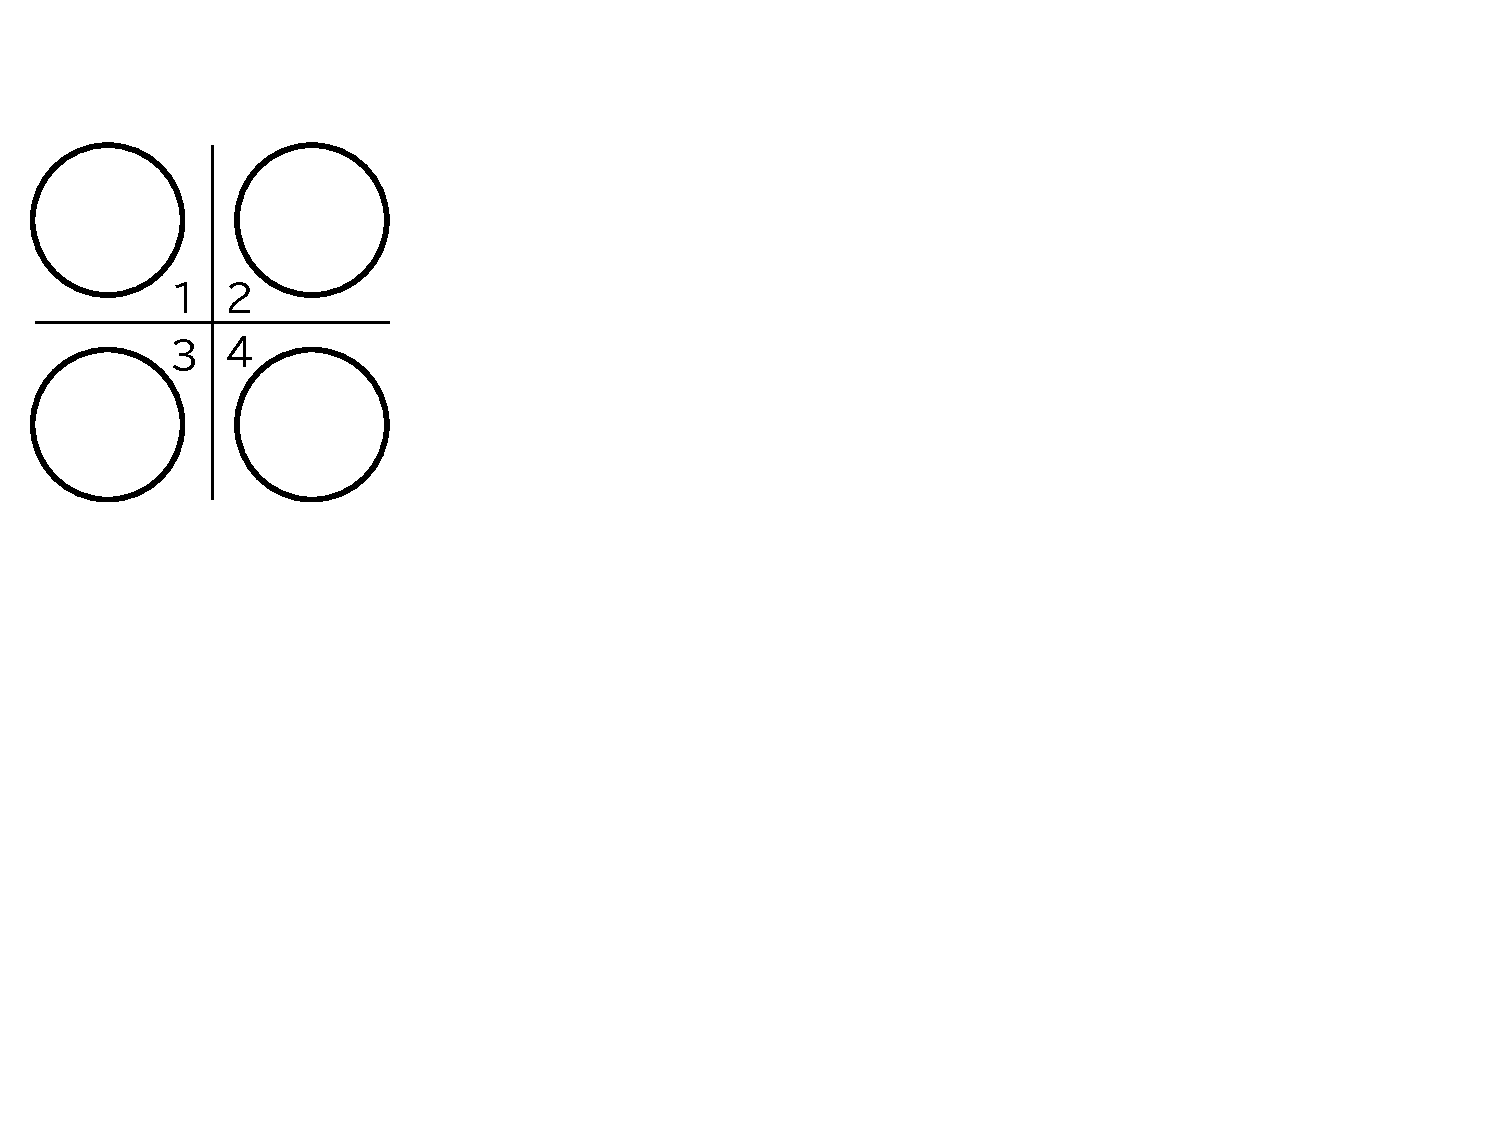
\includegraphics[width=3cm]{f1.pdf}\end{wrapfigure}
\message{ !name(prob_resume.tex) !offset(-62) }
